\documentclass[11pt,a4paper]{article}
\usepackage[T1]{fontenc}
\usepackage[utf8]{inputenc}
\usepackage{lmodern}
\usepackage[margin=25mm]{geometry}
\usepackage{amsmath,amssymb,amsthm,bm}
\setcounter{MaxMatrixCols}{12}
\usepackage{booktabs,longtable,array}
\usepackage{float}
\usepackage{graphicx,tikz}
\usetikzlibrary{arrows.meta}
\usepackage[numbers,sort&compress]{natbib}
\usepackage{microtype}
\usepackage[colorlinks=true,linkcolor=blue!45!black,citecolor=blue!45!black,
 urlcolor=blue!45!black]{hyperref}
\usepackage{url}
\hypersetup{pdftitle={Unique spanning-tree families bound the static response of every complete four-state Markov network},pdfauthor={Xiaojian Zeng}}
\setlength{\parskip}{3pt}
\setlength{\parindent}{1.2em}
\newtheorem{theorem}{Theorem}
\newtheorem{lemma}{Lemma}
\DeclareMathOperator{\conv}{conv}
\DeclareMathOperator{\Cov}{Cov}
\newcommand{\U}{\mathcal U}
\newcommand{\T}{\mathcal T}
\newcommand{\one}{\mathbf 1}
\newcommand{\dd}{\mathrm d}
\title{Unique spanning-tree families bound the static response\protect\\
of every complete four-state Markov network}
\author{Xiaojian Zeng\\[3pt]
\small PBC School of Finance, Tsinghua University, 100190\\
\small \texttt{xiaojianzeng@foxmail.com}}
\date{}

\begin{document}
\maketitle
\begin{abstract}
The steady-state sensitivity of a Markov network admits a geometric
description in terms of families of directed spanning trees. Fancher and
Horowitz conjectured that families uniquely determined by their combined
directed-edge multiplicities suffice to bound every response. We prove
this containment for the complete four-state network, for all twelve
strictly positive finite transition rates and arbitrary signed
logarithmic rate perturbations. The result is stronger than a separate
convex decomposition for each perturbation: the entire matrix of rooted-tree
edge marginals has one decomposition, with weights independent of the
perturbation direction. A fixed rescaling by the stationary probabilities
reduces arbitrary rates to balanced flows. After symmetric traffic is
removed, every four-state residual flow belongs, up to relabeling, to one
nonnegative tournament cone. Within this cone, 93 cubic coefficient
matrices admit exact rational decompositions over the 346 unique families.
We give the complete finite certificate and two separately implemented
exact checkers. The construction makes the associated topological
covariance response bounds unconditional for complete four-state
networks, without detailed balance or a small-affinity assumption. It
does not establish the conjecture for general graphs or the attainability
of every point of the response hull.
\end{abstract}

\section{Introduction}

Transition rates determine how a stochastic kinetic network responds to
a changing control parameter. Even in a small network, nonequilibrium
circulation allows that response to depend on many rate ratios. Structural
constraints can nevertheless restrict sensitivity without selecting a
particular set of rates. The support bound of Owen and
Horowitz~\cite{OwenHorowitz2023}, for example, limits sensitivity when a
specified set of rates shares a multiplicative input. General static
response formulas express changes in stationary probabilities and
currents through reduced inverse matrices and projection
operators~\cite{AslyamovEsposito2024}. A different exact structure is the
affine dependence among steady currents when the controlled edges obey
an appropriate connectivity condition~\cite{DalCengio2025}.

Fancher and Horowitz~\cite{FancherHorowitz2026} proposed a joint geometric
description of stationary probability responses. A rooted spanning tree
contributes the sum of the logarithmic rate perturbations along its
edges. Choosing one tree for each root gives a tree family and an
associated response vector. The matrix-tree theorem yields a convex
representation using all families [their Eq.~(5)]. They conjectured
that one can retain only the \emph{uniquely constructable} families:
those determined uniquely by their full vector of directed-edge
multiplicities [their Eq.~(6)]. Their supplementary construction proves
the triangle case, while their four-state tests provide finite numerical
evidence. A proof for all positive four-state rates requires more than
additional samples.

Here we establish that full four-state statement, together with a common
decomposition of all rooted-tree edge marginals. The new step is a
nonnegative coefficient certificate after reduction to a balanced-flow
cone. The matrix-tree formula, vertex-dependent rescaling of outgoing
rates, and current conservation are established tools; the coefficient
decomposition is the additional ingredient. Because the same weights
work for every perturbation direction, the result controls the joint
response rather than only a selected scalar sensitivity. It removes the
conjectural premise of the covariance bounds in
Ref.~\cite{FancherHorowitz2026} for the complete four-state graph.

\section{Model, tree families, and the result}
\label{sec:model}

Consider states $0,1,2,3$ with one transition in each direction between
every pair. With columns indexed by the source state, the master
equation and its rates are
\begin{equation}
 \dot p=W(\lambda)p,\qquad
 W_{ij}(\lambda)=k_{ij}e^{\lambda d_{ij}}\quad(i\ne j),\qquad
 W_{jj}(\lambda)=-\sum_{i\ne j}W_{ij}(\lambda).
 \label{eq:model}
\end{equation}
All twelve $k_{ij}$ are strictly positive and finite. We set
$\sum_{i\ne j}k_{ij}=1$ by choosing the time unit at $\lambda=0$; no
constraint on this sum is imposed as $\lambda$ varies. The control
parameter $\lambda$ and its logarithmic rate slopes $d_{ij}\in[-1,1]$
are dimensionless. Detailed balance is not assumed. Irreducibility
gives a unique positive stationary vector $\pi(\lambda)$, normalized
by $\one^T\pi(\lambda)=1$. Write $\pi=\pi(0)$ and
\begin{equation}
 r_j=\left.\partial_\lambda\log\pi_j(\lambda)\right|_{\lambda=0}.
 \label{eq:r}
\end{equation}
This is an exact first derivative of the stationary state at an arbitrary
nonequilibrium base point. It is not a transient or finite-frequency response.

An inward tree rooted at $j$ has one outgoing edge from each other state
and a directed path from each state to $j$. Let $\T_j$ denote all such
trees. For a directed edge $e=(i,j)$, the arrow is $j\to i$ and its rate
is $k_e=k_{ij}$. Define
\begin{equation}
 k^T=\prod_{e\in T}k_e,\qquad
 \tau_j(k)=\sum_{T\in\T_j}k^T,\qquad
 H_{je}(k)=\frac{\sum_{T\in\T_j:e\in T}k^T}{\tau_j(k)}.
 \label{eq:tree}
\end{equation}
Thus $H$ is a $4\times12$ matrix of conditional edge-inclusion
probabilities. The matrix-tree expression
$\pi_j=\tau_j/\sum_\ell\tau_\ell$ gives
\begin{equation}
 r=Hd-\one(\pi^THd).
 \label{eq:tree-response}
\end{equation}

A family $\alpha=(T_0^\alpha,T_1^\alpha,T_2^\alpha,T_3^\alpha)$
chooses one tree per root. Its incidence matrix and total directed-edge
multiplicity are
\begin{equation}
 I^\alpha_{je}=\one_{\{e\in T_j^\alpha\}},\qquad
 m_e^\alpha=\sum_{j=0}^3 I^\alpha_{je}.
 \label{eq:unique}
\end{equation}
Let $\U$ contain exactly those families for which no distinct family has
the same twelve-component vector $m^\alpha$. Opposite arrows are distinct
coordinates. Each root has 16 trees, so there are $16^4=65\,536$ families.
Full enumeration gives 5955 multiplicity classes, of which 346 are
singletons. Appendix~\ref{app:certificate} fixes an explicit encoding
and gives the complete witness used below.

\begin{theorem}[Common marginal decomposition]
\label{thm:main}
For every strictly positive finite rate array $k$ on the complete
four-state graph, there are weights $\theta_\alpha(k)\ge0$,
$\alpha\in\U$, with $\sum_{\alpha\in\U}\theta_\alpha(k)=1$ such that
\begin{equation}
 H(k)=\sum_{\alpha\in\U}\theta_\alpha(k)I^\alpha.
 \label{eq:main}
\end{equation}
The weights depend only on the base-point rates. Consequently, for every
$d\in[-1,1]^{12}$, setting $G^\alpha=I^\alpha d$ gives
\begin{equation}
 r=\sum_{\alpha\in\U}\theta_\alpha(k)
       \bigl[G^\alpha-\one(\pi^TG^\alpha)\bigr]
 \ \in\ \conv\{G^\alpha-\one(\pi^TG^\alpha):\alpha\in\U\}.
 \label{eq:response-hull}
\end{equation}
\end{theorem}

The theorem concerns edge marginals, not a coupling of the complete
probability laws on $\T_j$. It also makes no assertion that every point
in the displayed hull is attained by finite positive rates. The proof
below constructs one valid set of weights at each base point.

\section{Reduction to one balanced-flow cone}
\label{sec:cone}

\subsection{A fixed stationary-flow rescaling}

At the base point set
\begin{equation}
 q_{ij}=k_{ij}\pi_j\quad(i\ne j).
 \label{eq:rescale}
\end{equation}
Stationarity says that the incoming and outgoing $q$ flows at every state
are equal. Every tree rooted at $j$ uses exactly one outgoing edge from
each state $\ell\ne j$, so
\begin{equation}
 q^T=\left(\prod_{\ell\ne j}\pi_\ell\right)k^T,
 \qquad H_{je}(q)=H_{je}(k).
 \label{eq:invariance}
\end{equation}
The factor cancels from the conditional tree distribution. Such
outgoing-rate rescalings are also discussed after Eq.~(5) of
Ref.~\cite{FancherHorowitz2026}. The advantage of the particular choice
\eqref{eq:rescale} is that $q$, regarded as a rate array, has uniform
stationary probabilities. Its four tree sums therefore agree:
$\tau_j(q)=\tau(q)$.

Only the base-point array is made balanced. The rescaling in a perturbed
family is $q_{ij}(\lambda)=\pi_j(0)k_{ij}e^{\lambda d_{ij}}$; the factor
$\pi_j(0)$ is held fixed. The array $q(\lambda)$ need not remain balanced.
Accordingly, all derivatives below are taken with respect to the twelve
independent directed rates before imposing balanced-flow coordinates.
The final centering in Eq.~\eqref{eq:response-hull} uses the original
$\pi$, not the uniform distribution of $q$.

\subsection{Residual support and tournament classification}

For every unordered pair put $s_{ij}=\min(q_{ij},q_{ji})>0$ and subtract
that amount from both directions. The residual is a nonnegative balanced
flow with at most one positive direction on each pair. It has no positive
edge between distinct strongly connected components. Indeed, a source
component in the acyclic condensation graph has zero incoming flow, so
conservation of its total flow forces zero outgoing flow. Removing that
component and repeating proves the claim.

A nontrivial residual component contains at least three vertices, since
an opposite pair cannot remain. Thus the nonzero residual support on four
vertices is either strongly connected on all four vertices or a directed
triangle plus an isolated vertex. If it is strongly connected, orient
missing pairs to complete a strongly connected tournament. For a triangle,
give the fourth vertex at least one incoming and one outgoing arrow.
The completed tournament is again strongly connected. If the residual
is zero, choose any strongly connected tournament. Added arrows carry
zero residual flow and do not remove any original positive rate.

There is only one isomorphism class of strongly connected four-vertex
tournaments. Every vertex has outdegree one or two, and the sum of the
outdegrees is six. Let the two outdegree-two vertices be $a,b$, with
$a\to b$. Vertex $a$ beats one low-degree vertex $c$ and loses to the
other, $d$. Vertex $b$ must beat both $c$ and $d$, and $c$ must beat $d$.
These choices determine all arrows. We use the representative
\begin{equation}
 0\to1,\quad1\to2,\quad2\to0,\quad
 0\to3,\quad3\to1,\quad2\to3.
 \label{eq:tournament}
\end{equation}
Let $A,B,C\ge0$ be the residual flows on $0\to1$, $2\to3$,
and $0\to3$, respectively. Conservation then fixes the residual flows
on $2\to0$, $3\to1$, and $1\to2$ to $A+C$, $B+C$, and $A+B+C$.
They are equivalently the coefficients of the three directed cycles
$0\to1\to2\to0$, $1\to2\to3\to1$, and
$0\to3\to1\to2\to0$ (Fig.~\ref{fig:cone}).

\begin{figure}[tb]
 \centering
 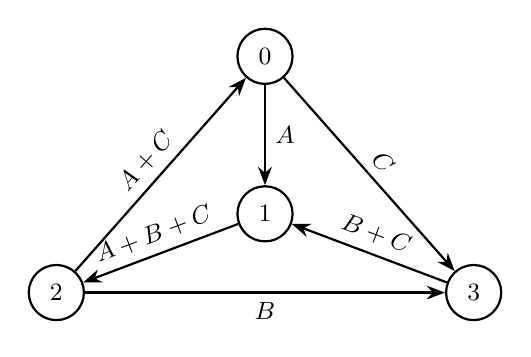
\begin{tikzpicture}[>=Stealth, line width=0.8pt,
  vertex/.style={circle,draw,fill=white,minimum size=7mm,inner sep=0pt},
  every edge/.style={draw,->}, every node/.style={font=\small}]
\node[vertex] (n0) at (0,3.0) {$0$};
\node[vertex] (n2) at (-2.65,0) {$2$};
\node[vertex] (n3) at (2.65,0) {$3$};
\node[vertex] (n1) at (0,1.0) {$1$};
\path (n0) edge node[right] {$A$} (n1)
      (n1) edge node[above,sloped] {$A+B+C$} (n2)
      (n2) edge node[above,sloped] {$A+C$} (n0)
      (n0) edge node[above,sloped] {$C$} (n3)
      (n3) edge node[above,sloped] {$B+C$} (n1)
      (n2) edge node[below] {$B$} (n3);
\end{tikzpicture}

 \caption{Canonical residual flow after removal of symmetric traffic.
 Arrow labels are flow magnitudes, with $A,B,C\ge0$.
 To recover the strictly positive rate array $q$, add $s_{ij}>0$ in
 both directions on each of the six pairs. Every balanced positive
 four-state array has this form after a state permutation; an arrow
 may have zero residual flow while both original rates remain positive.}
 \label{fig:cone}
\end{figure}

Thus every positive balanced array belongs, after relabeling, to the
following cone:
\begin{equation}
\begin{array}{c|ll}
 \{i,j\} & q_{ij}\ (i<j) & q_{ji}\ (i<j)\\\hline
 01 & s_{01} & s_{01}+A\\
 02 & s_{02}+A+C & s_{02}\\
 03 & s_{03} & s_{03}+C\\
 12 & s_{12} & s_{12}+A+B+C\\
 13 & s_{13}+B+C & s_{13}\\
 23 & s_{23} & s_{23}+B
\end{array}
\qquad s_{ij}>0,\quad A,B,C\ge0.
\label{eq:rates}
\end{equation}
This is a covering construction for arbitrary rates, including tied
opposite flows; it imposes no symmetry of the six $s_{ij}$. State
permutations act bijectively on families and on full multiplicity
classes, preserving membership in $\U$.

\section{The finite coefficient certificate}
\label{sec:certificate}

Let $x=(s_{01},s_{02},s_{03},s_{12},s_{13},s_{23},A,B,C)$.
After substituting Eq.~\eqref{eq:rates}, write
\begin{align}
 \tau_j(q(x))=\tau(x)&=\sum_{m\in\mathcal M}c_m x^m,
 \label{eq:tau-poly}\\
 N_{je}(x):=\left[q_e\frac{\partial\tau_j(q)}{\partial q_e}
                  \right]_{q=q(x)}
 &=\sum_{m\in\mathcal M}N_{m,je}x^m.
 \label{eq:n-poly}
\end{align}
The derivative in \eqref{eq:n-poly} marks an original directed edge,
not a cone variable. Every tree has three edges, so these polynomials
have degree exactly three. Direct expansion gives 93 nonzero monomials:
82 have $c_m=1$, ten have $c_m=2$, and $ABC$ has $c_m=3$.
All coefficients are nonnegative integers. The support of each numerator
is contained in that of $\tau$ because it sums a subset of the rooted
tree terms.

\begin{lemma}[Coefficient decomposition]
\label{lem:coeff}
For every $m\in\mathcal M$, there are nonnegative rational numbers
$\beta_{m,\alpha}$ supported on unique families such that
\begin{equation}
 \sum_{\alpha\in\U}\beta_{m,\alpha}=1,\qquad
 N_{m,je}=c_m\sum_{\alpha\in\U}\beta_{m,\alpha}I^\alpha_{je}
 \quad\text{for all }j,e.
 \label{eq:coeff}
\end{equation}
The complete witness in Table~\ref{tab:witness} uses $c_m$ families
for each monomial, each with weight $1/c_m$.
\end{lemma}

\begin{proof}[Finite exact verification]
The edge order and tree table in Appendix~\ref{app:certificate} decode
each listed family into its four trees. Enumerating all choices of one
tree per root and grouping by the full twelve-dimensional multiplicity
vector establishes the singleton status of every witness family.
Expanding each tree product with Eq.~\eqref{eq:rates} gives both $c_m$
and the marked-edge coefficient matrix $N_m$. For each row of
Table~\ref{tab:witness}, adding the listed family incidence matrices
gives exactly $N_m$, since the factor $c_m$ cancels the weight $1/c_m$.
This verifies all $93\times4\times12=4464$ component identities in
\eqref{eq:coeff}, together with positivity and normalization.

The accompanying programs perform this full finite calculation in
integer and rational arithmetic. One reconstructs trees by parent maps
and the polynomials from the $3\times3$ principal cofactors of the
column Laplacian $-W$. The other generates trees from Pr\"ufer sequences
and expands products by multisets of symmetric-flow and cycle labels.
Both regenerate all families and all nonzero monomials; neither assumes
the stored numerator matrices or singleton classifications are correct.
Only the proposed supports and rational weights are treated as witnesses
to be checked. Appendix~\ref{app:algorithm} states the verification
procedure and package interface. There is no floating tolerance or
truncation in these identities.
\end{proof}

\subsection{The coefficient of \texorpdfstring{$ABC$}{ABC}}

The only coefficient equal to three illustrates both the certificate
and its scope. In the directed-edge order
\begin{equation}
 E=(01,02,03,10,12,13,20,21,23,30,31,32),
 \qquad ij\equiv j\to i,
 \label{eq:edge-order}
\end{equation}
the marked-edge coefficient is
\begin{equation}
\setlength{\arraycolsep}{3pt}
 N_{ABC}=\begin{pmatrix}
0&3&0&0&0&3&0&3&0&0&0&0\\
0&2&0&2&0&3&0&0&0&1&0&1\\
0&0&0&2&0&3&0&3&0&1&0&0\\
0&1&0&1&0&0&0&3&0&2&0&2
\end{pmatrix}
 =I^{41333}+I^{41336}+I^{44990}.
\label{eq:abc}
\end{equation}
For root $0$, the residual support has the single tree
$\{2\to0,3\to1,1\to2\}$, whose product
$(A+C)(B+C)(A+B+C)$ has $ABC$ coefficient three. For root $1$,
the four possible tree products are
\begin{equation}
 A(A+C)(B+C),\quad AB(B+C),\quad
 C(A+C)(B+C),\quad CB(B+C).
 \label{eq:abc-trees}
\end{equation}
Their $ABC$ coefficients are $1,1,1,0$. The certificate uses twice
the tree associated with the first product and once the tree associated
with the fourth. These choices preserve every edge marginal, as
\eqref{eq:abc} shows, but change the full tree distribution of this
coefficient. The construction therefore must not be interpreted as
reproducing the complete rooted-tree laws. That stronger interpretation
is unnecessary for $G_j^\alpha$, which is linear in the edge indicators.
This example does not exclude a different full-law construction.

\section{Constructing the weights and bounding response}
\label{sec:weights}

For any cone coordinates representing a positive balanced flow, define
\begin{equation}
 \rho_m(x)=\frac{c_mx^m}{\tau(x)},\qquad
 \theta_\alpha(x)=\sum_{m\in\mathcal M}\rho_m(x)\beta_{m,\alpha}.
 \label{eq:weights}
\end{equation}
All $\rho_m$ are nonnegative and their sum is one. The denominator is
strictly positive, since all original $q_{ij}$ are positive; equivalently,
the positive symmetric traffic already supplies positive tree products.
Hence all $\theta_\alpha$ are nonnegative and normalized, even when one
or more of $A,B,C$ vanish. Dividing \eqref{eq:coeff} by $\tau(x)$ and
summing with $x^m$ gives
\begin{equation}
 H_{je}(q)=\frac{N_{je}(x)}{\tau(x)}
     =\sum_{\alpha\in\U}\theta_\alpha(x)I^\alpha_{je}.
 \label{eq:finish}
\end{equation}
Transport these family labels back through the state permutation used
in Sec.~\ref{sec:cone}. Equation~\eqref{eq:invariance} proves
\eqref{eq:main} for the original $k$. Multiplication by $d$ and subtraction
of the original $\pi$ mean in \eqref{eq:tree-response} prove
\eqref{eq:response-hull}. This completes the proof of
Theorem~\ref{thm:main}.

No exchange of a singular rate limit is involved. A choice of tournament
can change at a zero residual-current boundary, but the theorem requires
existence of weights at each base point, not a globally smooth selection.
In a chosen canonical cone the displayed certificate uses 78 distinct
unique families; the full set of 346 is retained in the invariant
statement. Under a common rate rescaling, all cubic monomials and
$\tau$ acquire the same factor, leaving the weights unchanged.

For a fixed state observable $Q=(Q_0,Q_1,Q_2,Q_3)$, let
$\langle Q\rangle_\pi=\sum_j\pi_jQ_j$ and
$\Cov_\pi(Q,G)=\langle QG\rangle_\pi-\langle Q\rangle_\pi
\langle G\rangle_\pi$. The observable itself is assumed independent
of $\lambda$. Then
\begin{align}
 \left.\partial_\lambda\langle Q\rangle_{\pi(\lambda)}\right|_0
 &=\sum_{\alpha\in\U}\theta_\alpha(k)\Cov_\pi(Q,G^\alpha),
 \label{eq:covmix}\\
 \min_{\alpha\in\U}\Cov_\pi(Q,G^\alpha)
 &\le\left.\partial_\lambda\langle Q\rangle_{\pi(\lambda)}\right|_0
 \le\max_{\alpha\in\U}\Cov_\pi(Q,G^\alpha).
 \label{eq:bounds}
\end{align}
The bound formula is the specialization of Eq.~(8) of
Ref.~\cite{FancherHorowitz2026}; the contribution here is a proof of its
underlying unique-family containment for all positive complete
four-state networks. At a specified base point the extrema require a
finite comparison over the 346 families. Their values still depend on
$\pi$, $Q$, and $d$; the theorem does not eliminate that physical
dependence or assert finite-rate saturation of an extremum.

The dimensions are consistent throughout: $k$, $q$, $s$, and the cycle
flows have units of inverse time; $\tau$ and $N$ have units of inverse
time cubed. The quantities $H$, $\rho$, $\theta$, $r$, $d$, and $\lambda$
are dimensionless. Equation~\eqref{eq:bounds} consequently has the
units of $Q$. This finite-state model has no spatial boundary or
infinite-dimensional tail to truncate.

\section{Verification, comparison, and limitations}

The universal rate quantifier is carried by the analytic reduction and
the complete finite polynomial identities. Additional exact rate tests
check the convention map and the implementation. The Pr\"ufer checker
reconstructs 210 positive-rate cases, including all 24 state permutations
for each zero/nonzero pattern of $A,B,C$, nonuniform stationary
probabilities, and a finite rate ratio $10^{36}$. For every case it
compares the complete marginal matrix and the twelve independent
response directions against exact row-generator linear solves. It also
enumerates all 64 tournaments and all $3^6=729$ residual directional
supports; all 75 possible positive supports of balanced flows are contained in the
24 relabelings of \eqref{eq:tournament}. These finite checks supplement
the analytic coverage argument; no sample count is used as evidence
for an untested continuum of rates.

The published two-state single-binding specialization of
Ref.~\cite{OwenHorowitz2023}, $W_{10}=x$ and $W_{01}=1$, provides a
simple normalization check. Direct solution gives
$\pi_1=x/(1+x)$, $\partial_{\log x}\pi_1|_{x=1}=1/4$, and effective
Hill coefficient one. The triangle family counts are also recovered:
27 families and 11 singletons, as in Ref.~\cite{FancherHorowitz2026}.
These are reproduced baselines, not additional results of this paper.

The general inverse/projection formulas of
Ref.~\cite{AslyamovEsposito2024}, Eqs.~(6)--(8) of its cited preprint
version, compute static response but do not supply the nonnegative
unique-family coefficients used here. The affine current relation of
Ref.~\cite{DalCengio2025}, Eq.~(7) of its cited preprint version, assumes
that deleting the controlled input edges leaves a connected graph;
its coefficients are not specified as nonnegative normalized weights.
It is a different statement from the simultaneous directed-rate
probability-response decomposition \eqref{eq:main}. These comparisons
identify the concrete additional content relative to the displayed
prior formulas, without claiming an exhaustive exclusion of every
possible indirect derivation.

The proof is limited to the complete four-state graph with all twelve
rates strictly positive and finite. It does not resolve the general-graph
conjecture, establish full-hull attainability, or impose a complete
tree-law coupling. It concerns first-order static response at an
arbitrary base point, with no claim about higher derivatives or finite
perturbation errors. The result describes a stochastic model rather
than an experimentally identified biochemical mechanism. Within this
scope, the common convex weights give a constructive bridge from
continuous rate parameters to the finite unique-family response bounds.

\section*{Data and code availability}

The full rational certificate is included as
\texttt{supplement/certificate.json}; its complete mathematical content
is tabulated in Appendix~\ref{app:certificate}. The accompanying
\texttt{check\_cofactors.py} and \texttt{check\_prufer.py} programs
reconstruct and verify the certificate using only the Python standard
library. The supplement provides execution instructions, conventions,
environment information, and table-regeneration code. No external
dataset, proprietary solver, or downloaded third-party code is needed
to check the finite identities.

\section*{Acknowledgements}

OpenAI Codex assisted the proof development, calculations, programming,
literature comparison, verification work, and manuscript drafting.
The model version identifiers remain unconfirmed. The reported
algebraic checks are reproducible integer and rational computations;
AI-assisted review is not external peer review or human author approval.

\clearpage
\appendix
\section{Complete certificate and decoding conventions}
\label{app:certificate}

Number the twelve directed edges from $0$ to $11$ in the order
\eqref{eq:edge-order}. At each root, sort the three edge indices within
each inward tree, then sort the resulting triples lexicographically.
The tree index $t$ runs from $0$ to $15$. Table~\ref{tab:trees} lists
all these triples. A family's integer ID is
\begin{equation}
 f=16^3t_0+16^2t_1+16t_2+t_3.
 \label{eq:family-id}
\end{equation}
The root labels are part of this definition: exchanging two trees
between roots is not an allowed identification. Uniqueness is checked
against all $65\,536$ IDs using their full directed-edge multiplicities.

\begin{table}[H]
\centering
\caption{Complete rooted-tree encoding. Each entry is a triple of
zero-based directed-edge indices, not a triple of vertex labels.}
\label{tab:trees}
\begin{tabular}{rcccc}
\toprule
$t$ & Root $0$ & Root $1$ & Root $2$ & Root $3$ \\
\midrule
0 & $0,1,2$ & $1,2,3$ & $0,2,6$ & $0,1,9$ \\
1 & $0,1,5$ & $1,3,5$ & $0,5,6$ & $0,4,9$ \\
2 & $0,1,8$ & $1,3,8$ & $0,6,8$ & $0,6,11$ \\
3 & $0,2,4$ & $1,5,9$ & $0,8,9$ & $0,9,11$ \\
4 & $0,2,11$ & $2,3,4$ & $2,3,7$ & $1,3,10$ \\
5 & $0,4,5$ & $2,3,11$ & $2,6,7$ & $1,7,9$ \\
6 & $0,4,8$ & $2,4,6$ & $2,6,10$ & $1,9,10$ \\
7 & $0,5,11$ & $3,4,5$ & $3,5,7$ & $3,4,10$ \\
8 & $1,2,7$ & $3,4,8$ & $3,7,8$ & $3,7,11$ \\
9 & $1,2,10$ & $3,5,11$ & $3,8,10$ & $3,10,11$ \\
10 & $1,5,7$ & $4,5,6$ & $5,6,7$ & $4,6,10$ \\
11 & $1,7,8$ & $4,5,9$ & $5,7,9$ & $4,9,10$ \\
12 & $1,8,10$ & $4,6,8$ & $6,7,8$ & $6,7,11$ \\
13 & $2,4,10$ & $4,8,9$ & $6,8,10$ & $6,10,11$ \\
14 & $2,7,11$ & $5,6,11$ & $7,8,9$ & $7,9,11$ \\
15 & $2,10,11$ & $5,9,11$ & $8,9,10$ & $9,10,11$ \\
\bottomrule
\end{tabular}

\end{table}

Table~\ref{tab:witness} specifies every nonzero monomial in
\eqref{eq:tau-poly}, its scalar coefficient, and the unique-family
support of its convex coefficient decomposition. All unlisted cubic
monomials have zero coefficient. Each listed family has weight $1/c_m$,
and all other $\beta_{m,\alpha}$ are zero. Thus the table and the
tree decoder specify the full finite witness without requiring a
particular numerical solver or an omitted coefficient file.

\begingroup
\small
\setlength{\tabcolsep}{10pt}
\begin{longtable}{lrrl}
\caption{Complete coefficient witness. Every listed family receives weight $1/c_m$; unlisted families receive zero. IDs use Eq.~\eqref{eq:family-id}.}\label{tab:witness}\\
\toprule $x^m$ & $c_m$ & Family IDs & Each weight \\ \midrule
\endfirsthead
\multicolumn{4}{c}{Table \thetable\ continued}\\
\toprule $x^m$ & $c_m$ & Family IDs & Each weight \\ \midrule
\endhead
\midrule\multicolumn{4}{r}{Continued on next page}\\
\endfoot
\bottomrule
\endlastfoot
$C^{3}$ & 1 & 41909 & $1$ \\
$B\,C^{2}$ & 2 & 41909, 44990 & $1/2$ \\
$B^{2}\,C$ & 1 & 44990 & $1$ \\
$A\,C^{2}$ & 2 & 41333, 41909 & $1/2$ \\
$A\,B\,C$ & 3 & 41333, 41336, 44990 & $1/3$ \\
$A\,B^{2}$ & 1 & 43384 & $1$ \\
$A^{2}\,C$ & 1 & 41333 & $1$ \\
$A^{2}\,B$ & 1 & 41336 & $1$ \\
$s_{23}\,C^{2}$ & 1 & 49134 & $1$ \\
$s_{23}\,B\,C$ & 1 & 49134 & $1$ \\
$s_{23}\,A\,C$ & 2 & 45806, 47496 & $1/2$ \\
$s_{23}\,A\,B$ & 1 & 47496 & $1$ \\
$s_{23}\,A^{2}$ & 1 & 45704 & $1$ \\
$s_{13}\,C^{2}$ & 1 & 41910 & $1$ \\
$s_{13}\,B\,C$ & 1 & 44991 & $1$ \\
$s_{13}\,A\,C$ & 2 & 41332, 41910 & $1/2$ \\
$s_{13}\,A\,B$ & 1 & 43385 & $1$ \\
$s_{13}\,A^{2}$ & 1 & 41332 & $1$ \\
$s_{13}\,s_{23}\,C$ & 1 & 53247 & $1$ \\
$s_{13}\,s_{23}\,A$ & 1 & 51609 & $1$ \\
$s_{12}\,C^{2}$ & 1 & 43957 & $1$ \\
$s_{12}\,B\,C$ & 1 & 43966 & $1$ \\
$s_{12}\,A\,C$ & 1 & 42869 & $1$ \\
$s_{12}\,A\,B$ & 1 & 42872 & $1$ \\
$s_{12}\,s_{23}\,C$ & 1 & 48622 & $1$ \\
$s_{12}\,s_{23}\,A$ & 1 & 47240 & $1$ \\
$s_{12}\,s_{13}\,C$ & 1 & 43963 & $1$ \\
$s_{12}\,s_{13}\,A$ & 1 & 42871 & $1$ \\
$s_{03}\,C^{2}$ & 1 & 33717 & $1$ \\
$s_{03}\,B\,C$ & 2 & 33717, 61374 & $1/2$ \\
$s_{03}\,B^{2}$ & 1 & 61374 & $1$ \\
$s_{03}\,A\,C$ & 2 & 32837, 33717 & $1/2$ \\
$s_{03}\,A\,B$ & 2 & 33717, 58702 & $1/2$ \\
$s_{03}\,A^{2}$ & 1 & 32837 & $1$ \\
$s_{03}\,s_{23}\,C$ & 1 & 61422 & $1$ \\
$s_{03}\,s_{23}\,B$ & 1 & 61422 & $1$ \\
$s_{03}\,s_{23}\,A$ & 1 & 58862 & $1$ \\
$s_{03}\,s_{13}\,C$ & 1 & 37814 & $1$ \\
$s_{03}\,s_{13}\,B$ & 1 & 65471 & $1$ \\
$s_{03}\,s_{13}\,A$ & 1 & 37814 & $1$ \\
$s_{03}\,s_{13}\,s_{23}$ & 1 & 65535 & $1$ \\
$s_{03}\,s_{12}\,C$ & 1 & 35765 & $1$ \\
$s_{03}\,s_{12}\,B$ & 1 & 60350 & $1$ \\
$s_{03}\,s_{12}\,A$ & 1 & 33861 & $1$ \\
$s_{03}\,s_{12}\,s_{23}$ & 1 & 60910 & $1$ \\
$s_{03}\,s_{12}\,s_{13}$ & 1 & 56251 & $1$ \\
$s_{02}\,C^{2}$ & 1 & 41893 & $1$ \\
$s_{02}\,B\,C$ & 2 & 41893, 44716 & $1/2$ \\
$s_{02}\,B^{2}$ & 1 & 44716 & $1$ \\
$s_{02}\,A\,C$ & 1 & 41381 & $1$ \\
$s_{02}\,A\,B$ & 1 & 41388 & $1$ \\
$s_{02}\,s_{23}\,C$ & 1 & 48844 & $1$ \\
$s_{02}\,s_{23}\,B$ & 1 & 48844 & $1$ \\
$s_{02}\,s_{23}\,A$ & 1 & 45772 & $1$ \\
$s_{02}\,s_{13}\,C$ & 1 & 41894 & $1$ \\
$s_{02}\,s_{13}\,B$ & 1 & 44717 & $1$ \\
$s_{02}\,s_{13}\,A$ & 1 & 41380 & $1$ \\
$s_{02}\,s_{13}\,s_{23}$ & 1 & 52957 & $1$ \\
$s_{02}\,s_{12}\,C$ & 1 & 43685 & $1$ \\
$s_{02}\,s_{12}\,B$ & 1 & 43692 & $1$ \\
$s_{02}\,s_{12}\,s_{23}$ & 1 & 48332 & $1$ \\
$s_{02}\,s_{12}\,s_{13}$ & 1 & 43690 & $1$ \\
$s_{02}\,s_{03}\,C$ & 1 & 33621 & $1$ \\
$s_{02}\,s_{03}\,B$ & 1 & 33621 & $1$ \\
$s_{02}\,s_{03}\,A$ & 1 & 32853 & $1$ \\
$s_{02}\,s_{03}\,s_{13}$ & 1 & 37734 & $1$ \\
$s_{02}\,s_{03}\,s_{12}$ & 1 & 34389 & $1$ \\
$s_{01}\,C^{2}$ & 1 & 4464 & $1$ \\
$s_{01}\,B\,C$ & 2 & 4472, 31091 & $1/2$ \\
$s_{01}\,B^{2}$ & 1 & 31096 & $1$ \\
$s_{01}\,A\,C$ & 1 & 4464 & $1$ \\
$s_{01}\,A\,B$ & 1 & 4472 & $1$ \\
$s_{01}\,s_{23}\,C$ & 2 & 8840, 31027 & $1/2$ \\
$s_{01}\,s_{23}\,B$ & 1 & 31112 & $1$ \\
$s_{01}\,s_{23}\,A$ & 1 & 8840 & $1$ \\
$s_{01}\,s_{13}\,C$ & 1 & 4468 & $1$ \\
$s_{01}\,s_{13}\,B$ & 1 & 31097 & $1$ \\
$s_{01}\,s_{13}\,A$ & 1 & 4468 & $1$ \\
$s_{01}\,s_{13}\,s_{23}$ & 1 & 31129 & $1$ \\
$s_{01}\,s_{12}\,C$ & 1 & 22385 & $1$ \\
$s_{01}\,s_{12}\,B$ & 1 & 22392 & $1$ \\
$s_{01}\,s_{12}\,s_{23}$ & 1 & 26760 & $1$ \\
$s_{01}\,s_{12}\,s_{13}$ & 1 & 22391 & $1$ \\
$s_{01}\,s_{03}\,C$ & 1 & 64 & $1$ \\
$s_{01}\,s_{03}\,B$ & 1 & 17731 & $1$ \\
$s_{01}\,s_{03}\,A$ & 1 & 64 & $1$ \\
$s_{01}\,s_{03}\,s_{23}$ & 1 & 17715 & $1$ \\
$s_{01}\,s_{03}\,s_{12}$ & 1 & 13377 & $1$ \\
$s_{01}\,s_{02}\,C$ & 1 & 4368 & $1$ \\
$s_{01}\,s_{02}\,B$ & 1 & 4370 & $1$ \\
$s_{01}\,s_{02}\,s_{23}$ & 1 & 8738 & $1$ \\
$s_{01}\,s_{02}\,s_{13}$ & 1 & 4372 & $1$ \\
$s_{01}\,s_{02}\,s_{03}$ & 1 & 0 & $1$ \\
\end{longtable}
\endgroup


\section{Exact checking and construction procedure}
\label{app:algorithm}

The following finite procedure verifies the coefficient lemma.
\begin{enumerate}
\item Generate every inward tree at each root and order them as in
Table~\ref{tab:trees}. Enumerate all four-tuples, compute their twelve
directed-edge multiplicities, and retain the singleton classes.
\item Construct each $\tau_j$ either as the sum of its tree products
or as a principal cofactor of $-W$. Form $q_e\partial_{q_e}\tau_j$
in twelve independent variables before applying \eqref{eq:rates}.
\item Expand all polynomials exactly in the nine cone variables.
Check equality of the four denominators, their complete monomial
support, and all scalar coefficients in Table~\ref{tab:witness}.
\item Decode every witness ID, check singleton membership and rational
weight normalization, and compare all 48 entries of \eqref{eq:coeff}
for each of the 93 monomials.
\end{enumerate}
The two packaged checkers use different tree and polynomial
representations for these steps. Both use integer polynomial
coefficients and \texttt{fractions.Fraction}; floating-point linear
programming was used only to discover candidate supports, which were
then rationally verified. The exact degree-three bound follows from
three-edge trees, not a fitted degree estimate.

To construct the response weights for a specified positive array, solve
$W\pi=0$ with $\one^T\pi=1$, set $q_{ij}=k_{ij}\pi_j$, and find a
state permutation whose canonical tournament contains every positive
residual arrow. At most 24 permutations need to be considered. Read
$s_{ij}$ and $A,B,C$ from \eqref{eq:rates}, evaluate \eqref{eq:weights},
and map each family back to the original state labels. This construction
uses no optimization over $d$.

The supplied checkers accept no numerical tolerance and terminate with
an error if a checked identity fails. They read the certificate relative
to their own location and write their result files in the current
working directory. Python 3.9.6 was used for the recorded checks; only
standard-library modules are required. The supplementary README gives
commands that can be run from an empty output directory. The analytic
rescaling and cone-coverage arguments remain part of the mathematical
proof and must be read together with the finite verification.

\begingroup
\raggedright
\bibliographystyle{unsrt}
\bibliography{references}
\endgroup
\end{document}
